\appendix

\section{Detailed Derivations}\label{appendix_derivations}

\subsection{Full-Order Model}

To obtain the full-order numerical solution, the governing equation is spatially discretized using variational principles of Discontinuous Galerkin (DG) to result in a high-dimensional system of ordinary differential equations (ODEs). The DG-FEM model is written in an element-wise form, which is beneficial for subsequent derivations of the lower-order models.Note that the choice of DG approach here is mainly for theoretical convenience in the subsequent coarse-graining formulation. In the numerical results, the full-order TPS ablation simulations is computed using standard FEM instead, and the equivalence between DG and standard FEM is noted upon their convergence.

\subsubsection{Domain Discretization}

Consider a conforming mesh partition of the domain, as shown in Fig.\hl{DOMAIN}, where each element belongs to one and only one component. Denote the collection of all $M$ elements as $\left\{E_i\right\}_{i=1}^{M}$. To ease the description of the DG model, a graph structure is employed. The elements are treated as vertices, the set of which is denoted $\cV=\left\{m\right\}_{m=1}^{M}$. Two neighboring elements, $E_i$ and $E_j$, are connected by an edge $(i,j)$, and the shared boundary between them is denoted $\eij$. The collection of all edges are denoted $\cE$, and $\cG$ is referred to as a graph. In the graph, the edges are unidirected, meaning if $(i,j)\in\cE$ then $(j,i)\in\cE$. Furthermore, denote the neighbors of the $i$-th element as $\cN_i=\left\{j | (i,j) \in\cE\right\}$. Lastly, for the ease of notation, introduce two special indices: $T$ for the boundary of an element that overlaps with the Dirichlet boundary condition, and similarly $q$ for the Neumann boundary condition.

\subsubsection{Weak Form of Discontinuous Galerkin Method}

Choosing appropriate basis functions $\phi_k$ and $\phi_l$ and using the Interior Penalty Galerkin (IPG) scheme ~\cite{Cohen and pernet 2018}, the variational bilinear form for \cref{eqn_thermal_pde} is,
\begin{equation}
    \sum_{i=1}^{M}a_{\epsilon,i}(\phi_k,\phi_l) = \sum_{i=1}^{M}L_i(\phi_k)
\end{equation}
where $\epsilon$ is an user-specified parameter and,
\begin{subequations}
    \begin{align}
        a_{\epsilon,i}(\phi_k,\phi_l) &= \int_{E^{(i)}}\left(\rho c_p \phik \frac{\partial \phil}{\partial t} + \nabla \phik\cdot\left(\mathbf{k}\nabla \phil\right) - \rho c_p \phik \vv\cdot\nabla\phil\right)dE^{(i)}\\
        &= -\sum_{j\in\cN_i\cup\dirichletset}\int_{\eij}\average{\bk\nabla\phik\cdot n}\jump{\phil}d\eij + \epsilon\sum_{j\in\cN_i\cup\dirichletset}\int_{\eij}\average{\bk\nabla\phil\cdot n}\jump{\phik}d\eij \notag\\
        &+ \sigma\sumneighbordirichlet\int_{\eij}\jump{\phik}\jump{\phil}d\eij\\
        L_i(v) &= \epsilon\sumneighbordirichlet\int_{\eij}\left(\bk\nabla\phil\cdot n\right)T_b d\eij + \int_{\eiq}\phik q_b d\eiq + \sigma\int_{\eiT}\phik T_b d\eiT
    \end{align}
\end{subequations}
In the bi-linear form above, the notations $\jump{}$ and $\average{}$ are respectively the jumps and averages at the boundary $\eij$ share by two elements $E_i$ and $E_j$,
\[
    \jump{u} = u\big|_{E_i} - u\big|_{E_j},\quad \average{u} = \frac{1}{2}\left(u\big|_{E_i} + u\big|_{E_j}\right), \quad \text{for } x\in\eij = E_i\cap E_j
\]
Furthermore, in the bi-linear form, the terms associated with $\sigma$ are introduced to enforce the Dirichlet boundary conditions; $\sigma$ is a penalty factor whose value can depend on the size of an element. Depending on the choice of $\epsilon$, the bi-linear form corresponds to symmetric IPG ($\epsilon=-1$), non-symmetric IPG ($\epsilon=1$), and incomplete IPG ($\epsilon=0$). All these schemes are consistent with the original PDE and have similar convergence rate with respect to mesh size. In the following derivations, the case $\epsilon=0$ is chosen for the sake of simplicity.

\subsubsection{Discontinuous Galerkin Model}

Next, the DG-based model is written in an element-wise form. For the $i$-th element, use a set of $P$ trial functions to represent the temperature as in \cref{eqn_element_temperature}. Without loss of generality, the trial functions are assumed to be orthogonal, so that $\int_{E^{(i)}} \phii_k(x) \phii_l(x) dx = \left|\Ei\right|\delta_{kl}$, where $\left|\Ei\right|$ is the area $(n_d=2)$ or volume $(n_d=3)$ of the $i$-th element, and $\delta_{kl}$ is the Kronecker delta.

Using test functions same as trial functions, the dynamics $\vu^{(i)}$ is obtained by evaluating the element-wise bi-linear forms,
\begin{equation}
    a_{\epsilon,i}(\phik^{(i)},T^{(i)}) = L_i(\phik^{(i)}),\quad k=1,2,\dots,P
\end{equation}
The above procedure yields,
\begin{equation}
    \vA^{(i)}\dot{\vu}^{(i)} = \left(\vB^{(i)} + \vC^{(i)}(t)\right)\vui + \sumneighbordirichlet\left(\vB^{(i)}_{ij}\vui + \vB^{(j)}_{ij}\vuj\right) + \vf^{(i)}(t)\label{eqn_element_wise_model}
\end{equation}
where for $k,l=1,2,\dots,P$,
\begin{subequations}
    \begin{align}
        \left[\vA^{(i)}\right]_{kl} &= \intEi\rho c_p\phik^{(i)}\phil^{(i)}d\Ei\\
        \left[\vB^{(i)}\right]_{kl} &= -\intEi\left(\nabla\phik^{(i)}\right)\cdot\left(\vk\nabla\phil^{(i)}\right)d\Ei\\
        \left[\vC^{(i)}\right]_{kl} &= \intEi\rho c_p \phik^{(i)}\vv^{(i)}\cdot\nabla\phil^{(i)}d\Ei\\
        \left[\vBi_{ij}\right] &= \int_{\eij}\average{\vk\nabla\phik^{(i)}\cdot\hat{n}}\phil^{(i)} - \sigma\jump{\phik^{(i)}}\phil^{(i)}d\eij\\
        \left[\vBj_{ij}\right] &= \int_{\eij}-\average{\vk\nabla\phik^{(i)}\cdot\hat{n}}\phil^{(j)} + \sigma\jump{\phik^{(i)}}\phil^{(j)}d\eij\\
        \left[\vf^{(i)}\right]_k &= \int_{\eiq}\phik^{(i)}q_bd\eiq + \sigma\int_{\eiT}\phik^{(i)}d\eiT
    \end{align}
\end{subequations}
Note that the matrices $\vA^{(i)}$, $\vC^{(i)}$, and $\vB_{ij}$ depend on $\rho$, $c_p$, and $\vk$, respectively, and hence can be a non-linear function of $\vu$. Since the trial functions are orthogonal, if $\rho c_p$ is constant within an element, $\vAi$ is diagonal; otherwise, $\vA_i$ is symmetric and positive definite as $\rho c_p > 0$.

For compactness, the element-wise model in \cref{eqn_element_wise_model} is also written in matrix form,
\begin{equation}
    \vA(\dot{\vu}) = \left[\vB(\vu) + \vC(t,\vu)\right]\vu + \mathbf{f}(t)\label{eqn_complete_model}
\end{equation}
where $\vu = \left[\vu^{(1)},\vu^{(2)},\cdots,\vu^{(M)}\right]^T\in\mathbb{R}^{MP}$ includes all DG variables, $\vf=\left[\vf^{(1)},\vf^{(2)},\dots,\vf^{(M)}\right]^T\in\mathbb{R}^{MP}$, $\vA$ and $\vC$ are matrices of $M$ diagonal blocks whose $i$-th blocks are $\vAi$ and $\vCi$, and $\vB$ is a matrix of $M\times M$ blocks whose $(i,j)$-th block is,
\begin{equation}
    \vB_{ij} = \begin{cases}
            \vBi + \sumneighbordirichlet\vBi_{ij}, & i=j\\
            \vBj_{ij}, & i\neq j
        \end{cases}
\end{equation}
The dependency of $\vA$, $\vB$, and $\vC$ on $\vu$ is explicitly noted in \cref{eqn_complete_model}, which is the source of non-linearity in the current TPS problem. Moreover, the mesh velocity $\vv$ varies with space and time, and thus the advection matrix $\vC$ varies with time as a function of $q_b$.

\subsection{Lumped Capacitance Model}

The following assumptions are employed: (1) the temperature in component $(i)$ is described by a scalar time-varying average temperature $\bar{u}^{(i)}$, (2) between neighboring components $(i)$ and $(j)$ the heat flux is approximated as,
\begin{equation}
    q_{ij} = \frac{\baruj - \barui}{R_{ij}}
\end{equation}
where $R_{ij}$ is the thermal resistance. Empirically, for a component of isotropic heat conductivity $k$, length $\ell$, and cross-section area $A$, the thermal resistance is $R=\ell/kA$. Between components $i$ and $j$, define $R_{ij}=R_{i} + R_{j}$. In addition, the heat flux due to Dirichlet boundary condition is computed as $q_{iT} = (T_b - \barui)/R_{i}$.

At component $i$, the dynamics of LCM are given by,
\begin{subequations}
    \begin{align}
        \int_{\Ei}\rho c_p \dot{\bar{u}}^{(i)} d\Ei &= \left(\sumneighbori\int_{\eij}\frac{\baruj - \barui}{R_{ij}}d\eij\right) + \int_{\eiq} q_b d\eiq + \int_{\eiT}\frac{T_b - \barui}{R_i}d\eiT\label{eqn_lcm_1}\\
        \bar{A}^{(i)}\dot{\bar{u}}^{(i)} &= \left(\sumneighbori\frac{|\eij|}{R_{ij}}\left(\baruj - \barui\right)\right) + |\eiq|\bar{q}^{(i)} + \frac{|\eiT|}{R_i}\left(\bar{T}^{(i)} - \barui\right) \label{eqn_lcm_2}\\ 
        &= \sumneighbori\left(-\frac{|\eij|}{R_{ij}}\barui + \frac{|\eij|}{R_{ij}}\baruj\right) + \left(-\frac{|\eiT|}{R_{i}}\barui\right) + \left(|\eiq|\bar{q}^{(i)} + \frac{|\eiT|}{R_i}\bar{T}^{(i)}\right)\label{eqn_lcm_3}\\
        &= \sumneighbordirichlet\left(\bar{B}^{(i)}_{ij}\barui + \bar{B}^{(j)}_{ij}\baruj\right) + \bar{f}^{(i)}\label{eqn_lcm_4}
    \end{align}
\end{subequations}
where in \cref{eqn_lcm_2} $|e|$ denotes the length $(d=2)$ or area $(d=3)$ of a component boundary $e$. The $\bar{A}^{(i)}$, $\bar{B}_{ij}^{(i)}$, and $\bar{B}_{ij}^{(j)}$ quantities are provided in \cref{eqn_lcm_elements}.

The lumped-mass representation for the four-component TPS in Fig.~\ref{fig_lcm_domain} is shown in Fig.~\ref{fig_lumped_mass_representation}. Leveraging the formulas from \cref{eqn_lcm_matrices,eqn_lcm_matrices_elements}, the LCM model takes

\begin{figure}
    \centering
    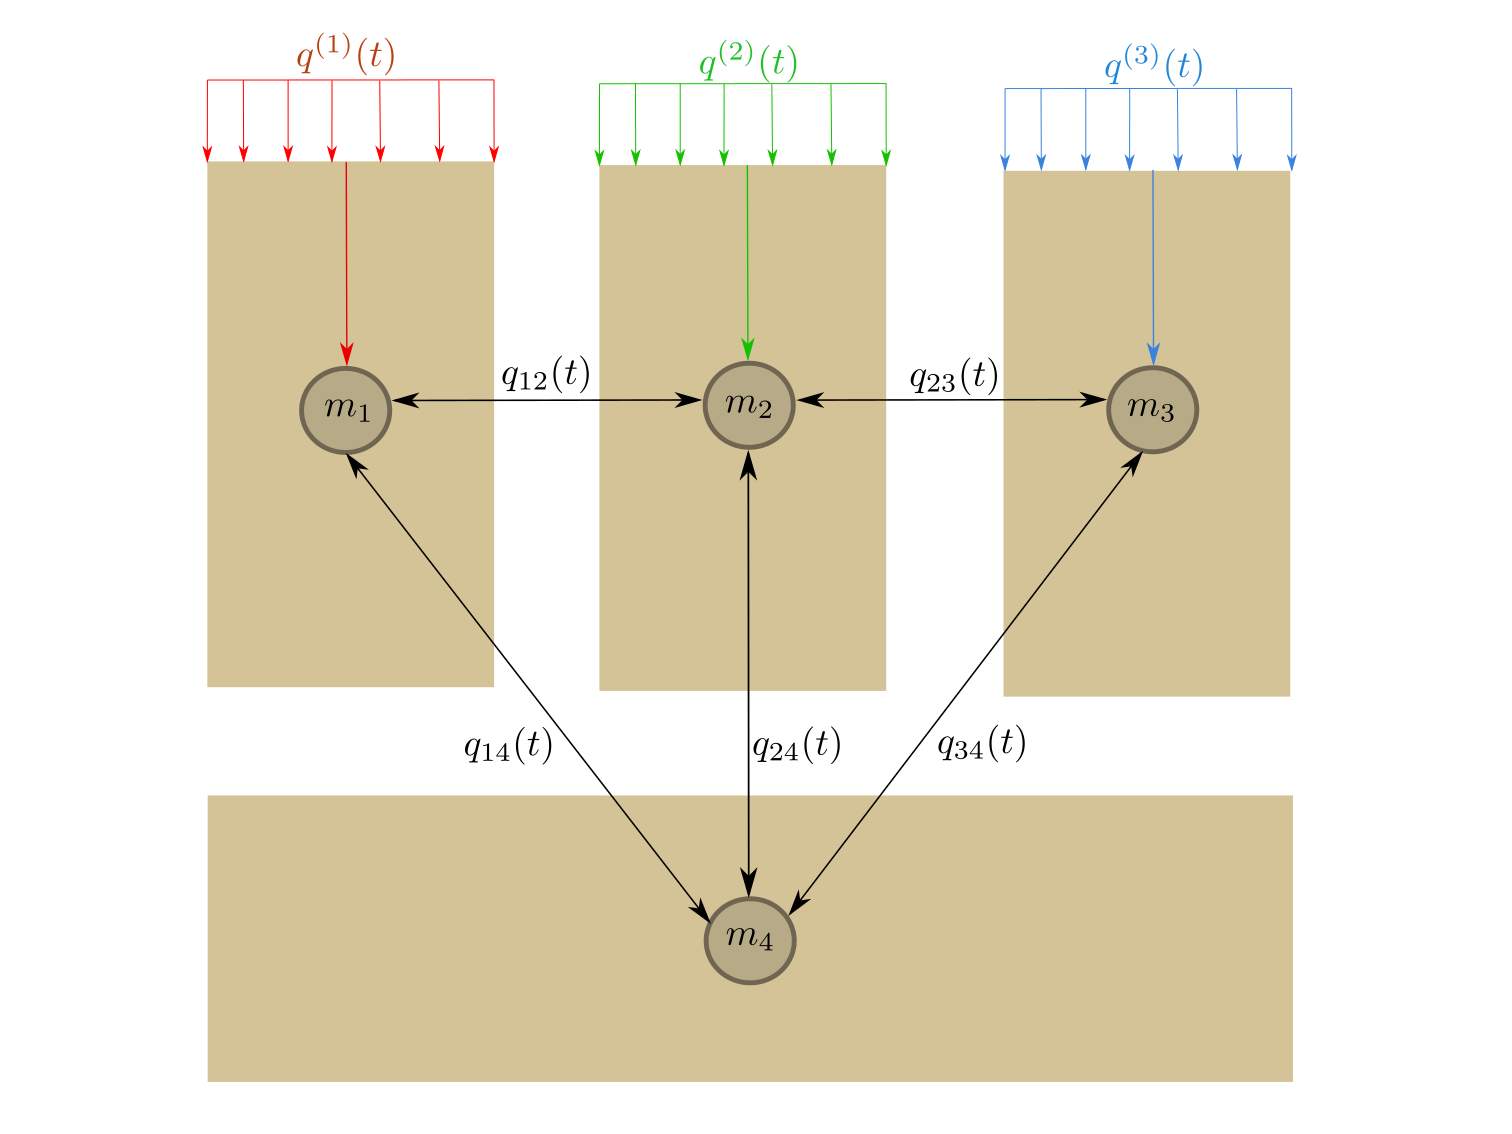
\includegraphics[width=0.5\textwidth]{./figs/lumped_mass_representation.png}
    \caption{Lumped mass representation for the four-component TPS.}
    \label{fig_lumped_mass_representation}
\end{figure}

